%!TEX TS-program = xelatex
\documentclass[11pt]{article}

\usepackage[a4paper,top=2cm, bottom=1.5cm, left=2cm, right=2cm]{geometry}

\usepackage{fontspec}
\usepackage{xeCJK} 
\usepackage{graphicx}
\usepackage{float}
\usepackage{multirow}

\XeTeXlinebreaklocale "zh"
\XeTeXlinebreakskip = 0pt plus 1pt
% \setCJKmainfont{LiHei Pro}
\setCJKmainfont{LiSong Pro}
\newfontfamily{\K}{LiHei Pro}

\newcommand{\todo}[1]{[{\color{red}{#1}}]}
\renewcommand{\figurename}{圖}
\renewcommand{\tablename}{表}

\begin{document}

\begin{center}{\Huge AlumniBook} {G3} \end{center}

\begin{center}
\begin{tabular}{cccc}
郗昀彥 R00725051&郭瀚智 R02725023&鄭立民 R02725041&李奕德 B99705021 \\
張凱涵 B00705027&施淮振 B00705047&倪嘉銘 T02705102&
\end{tabular}
\noindent\makebox[\linewidth]{\rule{\linewidth}{0.4pt}}
\end{center}

\tableofcontents

%% ++++++++++++++++++++++++++++++
\section{專案背景及目的}

本系在發展茁壯的同時培養了許多傑出的人才,這些人散布在各個不同領域。在超級專業化的現代若能連結正確領域的人來提供系上一些建議與幫助,必能讓資管系所內的課程內容與訓練更加的紮實。所以除了學生間的相互聯絡,本系統也將會提供系友與教授及行政人員進入本系統,對其所擅長之專業領域提供協助。學生亦可藉由本系統盡早深入了解產業現況,獲得更多正確且即時的資訊並對未來發展方向有更確實精確的判斷。

為了確保使用者身分得正確性,本系統必須要求使用者經由計算機中心(或其他認證機構)所提供的身分認證服務來認證使用者和其所宣稱的人為同一個人以防冒用。經正確認證之使用者於進入本系統後,會來到共用之瀏覽區。在這個區塊可以看到目前系統中的所有議題,瀏覽並參與討論。在觀看議題的同時使用者也可針對特定議題發表評論,此評論將會由任何觀看此議題的人共同看見。

在討論區中的所有議題都會根據其在發文時選擇的標籤做分類,方便其他使用者閱讀。使用者可以自由的訂閱包含特定標籤的議題,系統會再此類別議題建立時發信至使用者註冊時所使用得系信箱帳戶,讓使用者可以更密切的關柱該類別的議題。若只是關注特定議題之後續發展,亦可選擇只訂閱該議題。系統將依照使用者要求在此議題及其評論更新或新增時寄信至用戶信箱。另外,留言也會自動讓系統將該議題加入訂閱列表。

若在閱讀討論區時對特定人士產生興趣,也可以在適當的隱私權相關管理下查詢特定的系友的相關資訊。能否能夠看見該使用者所有相關資料取決於資料擁有者的個人隱私條件以及搜尋者之帳號類別,或是搜尋者與被搜尋者之間有在本系統中建立特別的朋友關係。本系統中若存在朋友關係則再搜尋時會由特定對象獨立於依照帳號類別做設計的隱私規則,直接套用該使用者針對朋友設定的隱私權相關設定,讓朋友間能夠更加深入的了解彼此。在好友關係尚未建立的情況下,使用者依然可以追蹤其他使用者,系統將會在該用戶發布新的議題時告知訂閱者這項訊息。

除了瀏覽討論區外,使用者亦可編輯自身的相關資料與隱私相關選項來讓自己被更多人看見。本系統將提供預先填入之公開資訊、基礎的個人連絡資訊輸入、以及與職業生涯相關之記錄,三個主要區塊。使用者可依照自身之習慣與想法選擇性的填入資料與決定其公開性。預設的群組別為校友、學生、教授及行政人員、與院系人員及朋友幾種,未來可再依據使用者需求做調整。

本系統旨在於建立一個能夠有效凝聚資管系所內之相關人士,提供一個跨界跨部(研究所與大學部)之溝通平台。本系統將階段性提供完整的溝通整合服務,冀望成為連結具專業知識的人幫忙解答疑惑,也希望能夠成為校友找人、學生找事之合作橋梁。

%% ++++++++++++++++++++++++++++++
\section{專案假設與限制}

為使本計畫順暢運行,其執行環境必須具有以下幾點之限制,其中缺乏任一一項將造成時程延宕或效果不如預期等等缺陷。

\begin{itemize}
\item{[身分認證]~~關於身分認證部分,台大計算機中心必須能夠提供 single sign-on 之服務,並且能夠回應本系統所有身分認證之需求。同時,回傳之 token 必須包含學號等資訊以供系統自動填入使用者帳號詳細內容使用。}
\item{[硬體]~~台大資管系必須能夠提供用於最後架站所需之伺服器的硬體設備或虛擬伺服器。}
\item{[帳戶資料]~~台大資管系必須提供預設帳戶之資料,以供建立初始使用者名單之用。或系所應能提供學號之判別方式來認證所有正常的用戶,例如其學號範圍、數字上的特徵與限制等等。}
\item{[使用者習慣討論]~~本系統需能夠對隸屬於每個不同預設分類項下之使用者做指定形式之訪談,以便了解每個職位之使用者對本系統之期望與意見。此意見將影響預設帳號類別之新增與刪去、朋友關係的用途與系統未來發展之用。}
\item{[階段性開放]~~本計畫將以階段性的方式向終點努力,期間所釋出的測試系統並不一定與完成系統之表現、內容完全相同。會依照以下順序依序開放測試:
\begin{itemize}
\item{使用者帳號管理}
\item{討論區測試}
\item{完整上線系統}
\end{itemize}}
\item{[使用者範圍]~~本系統預設之使用者範圍為校友、學生、教授及行政人員。超出本規畫範圍者將必須等到完整系統上線後發現有必要才會以更新版本的新增。}
\item{[行動裝置]~~本系統雖有預設API開放給未來發展之非特定行動裝置系統中的程式,但是並不包含強制性的程式開發,將再行有餘力之時完成此部分。}
\item{[電子郵件服務]~~台大資管系在軟硬體準備時必須開起電子郵件服務,讓本系統能順暢得依照使用者之要求處理訂閱議題以及類別之需求。}
\end{itemize}


%% ++++++++++++++++++++++++++++++
\section{專案範圍}

\subsection{功能性需求}
在功能性需求的部分本系統應包含登入模組、個人資料管理模組、討論區模組、搜尋模組、關係建立模組、行動裝置模組、討論區模組、訂閱模組、使用者列表模組、首頁模組。全部功能性需求請見表~\ref{req}。

\begin{table}[t]
\centering
\begin{tabular}{ | l | l | l | }
\hline
功能模組 & 功能需求 & 功能範圍 \\ \hline \hline
\multirow{3}{*}{登入模組} 
& 輸入身分 & 讓使用者宣稱自己的身分\\
& 身分認證 & 透過計中做身分認證 \\
& 取得token & 回收計中回傳的 token \\ \hline
\multirow{6}{*}{個人資料管理模組} 
& 管理公開資料 & 讓使用者維護帳號的公開資訊 \\
& 管理個人聯絡資料& 讓使用者維護帳號的聯絡資料\\
& 職業生涯資料管理& 讓使用者維護職業生涯相關資料 \\
& 隱私權管理& 讓使用者管理帳號之公開性選項 \\
& 關係管理& 讓使用者管理與其他帳號之間的關係 \\
& 儲存資料異動& 儲存任何使用者新增/修改/刪除之資料 \\ \hline
\multirow{2}{*}{搜尋模組} 
& 搜尋特定使用者 & 依照指定學號搜尋符合帳號 \\
& 回傳指定使用者 & 依照指定學號回傳符合條件之帳號 \\ \hline
 \multirow{3}{*}{關係建立模組} 
& 傳送使用者好友要求 & 由被要求者決定是否成為該用戶之朋友 \\ 
& 記錄使用者對於要求之回應 & 提供被要求者回應交友要求 \\
& 記錄使用者與其他用戶之友好狀況 & 儲存所有與該使用者為好友關係的連結 \\ \hline
\multirow{4}{*}{討論區模組}
& 新增議題 & 讓使用者以自己的帳號新增議題 \\
& 瀏覽議題 & 讓使用者流覽系統中之議題 \\
& 標示議題類別 & 讓使用者清楚了解顯示的議題之標籤 \\
& 管理議題 & 系統管理者確認類別系統正常運作 \\ \hline
\multirow{3}{*}{訂閱模組}
& 訂閱使用者 & 讓使用者關注其他使用者在系統中的發文 \\
& 訂閱議題 & 讓使用者關注特定議題的後續發展 \\
& 訂閱議題類別 & 讓使用者關注特定議題類別的新增議題 \\ \hline
\multirow{2}{*}{使用者列表}
& 預設顯示模組 & 顯示系統內所有使用者之公開資料 \\
& 過濾模組 & 依照使用者需求過濾資料後顯示 \\ \hline
\multirow{2}{*}{首頁}
& 系統公告模組 & 顯示系統公告 \\
& 整合模組 & 連結系上公告 \\ \hline
\end{tabular}
\caption{功能性需求列表}
\label{req}
\end{table}

\subsection{非功能性需求}
非功能性需求的部分主要牽涉到關於資料未來可能的彈性、系統運作的穩定性、系統元件的重複利用可能、以及資訊安全等。
\begin{itemize}
\item{[資料可變性]~~針對例如說使用者種類或是文章類型等等資訊,設計出未來較容易擴充之資料儲存模型。 }
\item{[系統穩定性]~~硬體方面,需配置不斷電系統以及資料自動備份系統以維持系統不斷線的能力。另一方面,也需要設計具有平衡流量能力的伺服器架構,以有效降平均回應時間。}
\item{[系統安全性]~~軟體方面,為防止已知的幾種攻擊方式,本系統在設計時必須確保使用者不會再不恰當的地方使用”‘“等特殊符號。包含 SQL injection 在內的幾種攻擊方式都必須要在系統設計時避免。}
\item{[使用者期望]~~為確保本系統朝向正確且易學易用的方向發展,在發展過程中將不定期的針對特定使用者族群做抽樣調查。取得之資料將在適當的分析之後,用於增進系統效能與新增功能或是修改錯誤等等面向。}
\end{itemize}

%% ++++++++++++++++++++++++++++++
\section{解決方案}

\subsection{系統概述}

本系統包含兩個主要的使用情境:「使用者個人資訊與情報的建立與管理」以及「成員之間的互動論壇」。兩者之使用情境如圖~\ref{pic:use:userLogin} 與圖~\ref{pic:use:forum}。

\begin{figure}[H]
\centering
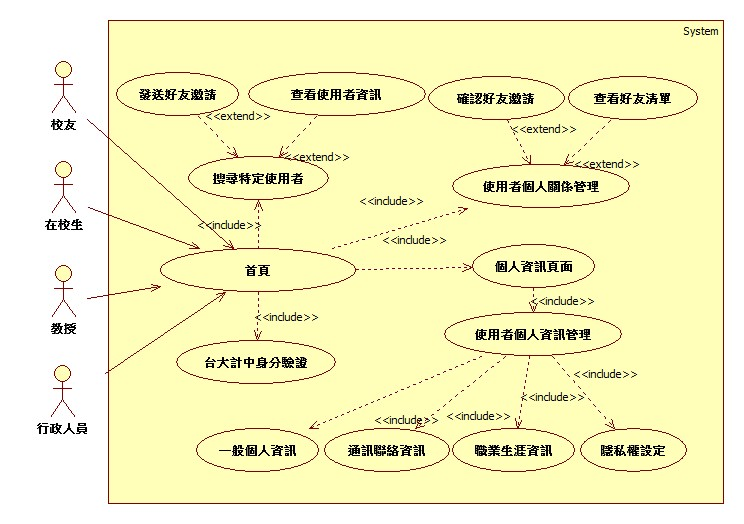
\includegraphics[width=.95\textwidth]{img/useseq/stage1/userProfile.jpg}
\caption{Use Case Diagram -- 使用者資訊管理}
\label{pic:use:userLogin}
\end{figure}

\begin{figure}[H]
\centering
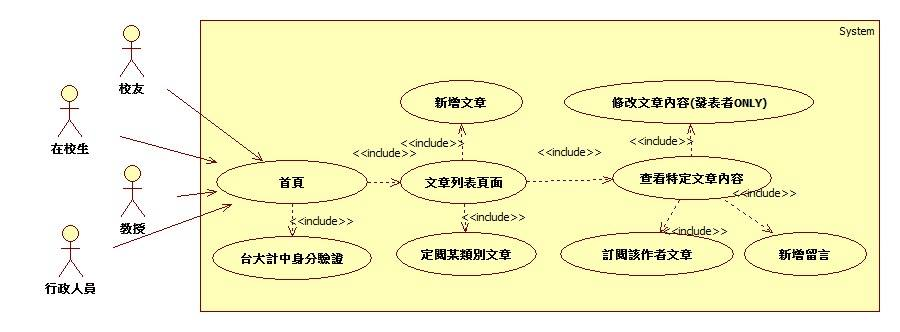
\includegraphics[width=1.05\textwidth]{img/useseq/stage2/useForum.jpg}
\caption{Use Case Diagram -- 文章與留言管理}
\label{pic:use:forum}
\end{figure}

以下之各小節將會逐一介紹各模組之功能及其設計概念。

%% ####################### %%
\subsubsection{登入模組}
在登入模組中需包含以下幾點功能: 
\begin{itemize}
\item{宣稱身分}
\item{身分認證}
\item{取得回傳之 token 並解構}
\end{itemize}
在宣稱身分的地方必須由使用者宣稱自己的身分並提供相關認證資料,在經由計算機中心所提供之 single sign-on 之服務完成身分認證之後,回傳給系統一組經認證的特定格式之 Token。若使用者為初次登入本系統,則此 Token 在經系統解構之後必須能夠抽取部分必要資料填入系統之資料庫中做為使用者個基礎資訊。此行為將於前端網頁系統中完成,若有需要填入時則會交由後端資料系統負責。使用者與系統之間的互動請參考圖~\ref{pic:seq:login}。

\begin{figure}[H]
\centering
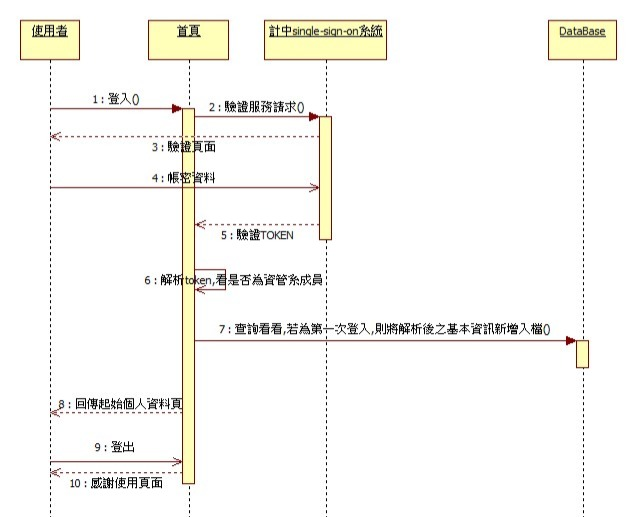
\includegraphics[width=.85\textwidth]{img/useseq/stage1/seqLogin.jpg}
\caption{Sequence Diagram -- 首頁登入}
\label{pic:seq:login}
\end{figure}

%% ####################### %%
\subsubsection{個人資料管理模組}

\begin{figure}[H]
\centering
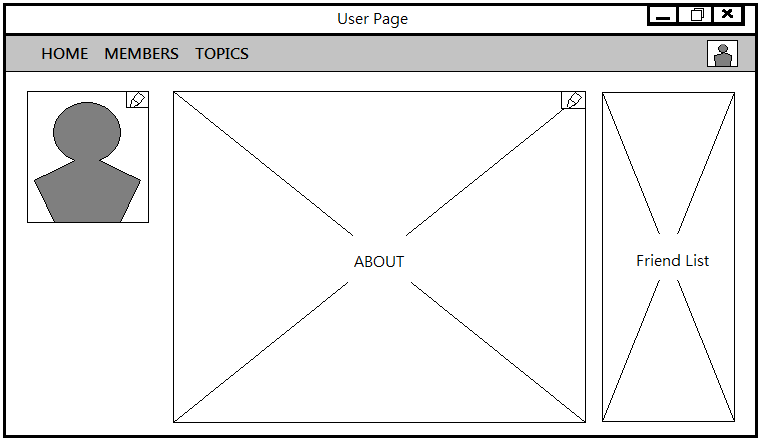
\includegraphics[width=0.7\textwidth]{img/prototype/UserPage.png}
\caption{Prototype -- 用戶資訊頁面}
\label{pic:pro:profile}
\end{figure}

個人資料管理模組將負責管理每個使用者各自的資料組,此資料組中包含使用者的公開資料、個人連絡資料、職業生涯相關資料與隱私權管理及關係管理。使用者必須能夠看見目前系統內的資料狀況並且能夠更動大部分的資料,其中如學號等等的則必須要經過系統管理者之認證後方可變更。此更改之行為將於前端網頁系統中完成,若有資料必須儲存則會交由後段資料系統負責。使用者與系統之間的互動請參考圖~\ref{pic:seq:profileMgt}。此功能會產生一系列之獨立頁面以便於瀏覽與修改個人資訊,雛形如圖~\ref{pic:pro:profile} 所示。

\begin{figure}[H]
\centering
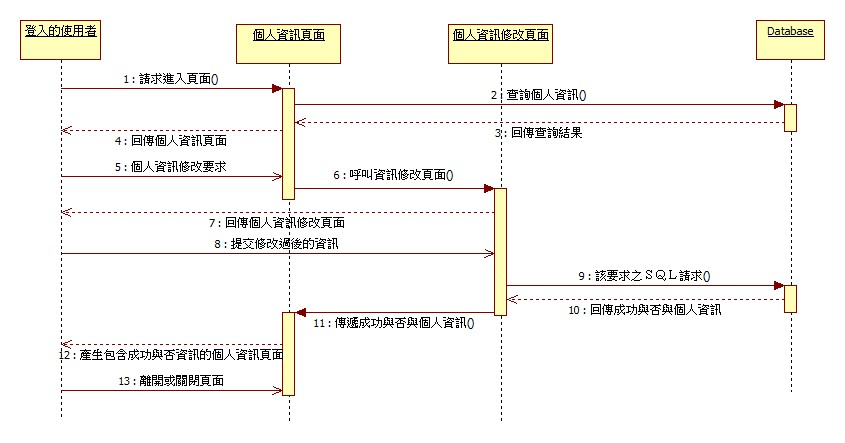
\includegraphics[width=\textwidth]{img/useseq/stage1/seqProfileEdit.jpg}
\caption{Sequence Diagram -- 個人資訊管理與個人資訊修改}
\label{pic:seq:profileMgt}
\end{figure}

%% ####################### %%
\subsubsection{搜尋模組}
本系統為了建立一個適合使用者相互溝通之平台,必須提供使用者方便互相連結之功能,搜尋模組正是為了此需求所建立。當使用者在討論區中產生對特定用戶之好奇心,便可藉由本模組使用特定資料(如:學號)做為索引找到該用戶之公開資訊。公開程度將依該用戶之隱私設定做限制,若該用戶認為預設之帳號類別方式無法達成所欲之特殊公開之組合則需透過朋友關係的建立來達成要求。互相成為朋友的兩人將以特別規則優於普通規則的方式優先採用該用戶所設定的特別規則觀看公開資訊。本搜尋功能將全部於前端網頁系統完成。使用者與系統之間的互動模式請參考圖~\ref{pic:seq:searchUser} ,可產出之相對網頁原形 (prototype) 如圖~\ref{pic:pro:memberList} 。

除了使用者搜尋之外,如圖~\ref{pic:use:forum} 中的「文章列表頁面」以及「查看特定文章內容」等部分所描述之情境,系統也允許使用者針對文章或是文章分類去進行搜尋。與此功能相對之網頁原形 (prototype) 如圖~\ref{pic:pro:articleList} 。

\begin{figure}[H]
\centering
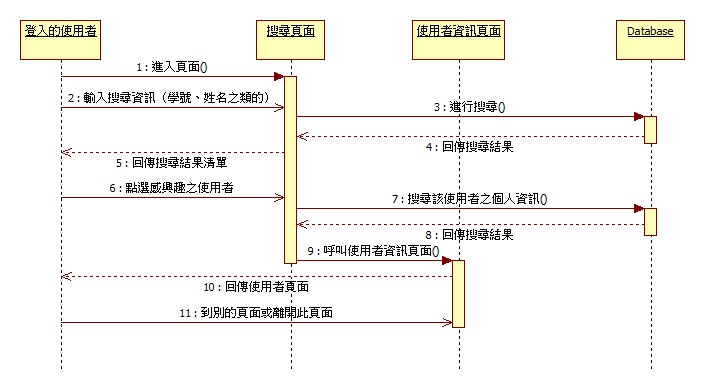
\includegraphics[width=\textwidth]{img/useseq/stage1/seqSeqrchUser.jpg}
\caption{Sequence Diagram -- 搜尋查看他人使用者資訊}
\label{pic:seq:searchUser}
\end{figure}

\begin{figure}[H]
\centering
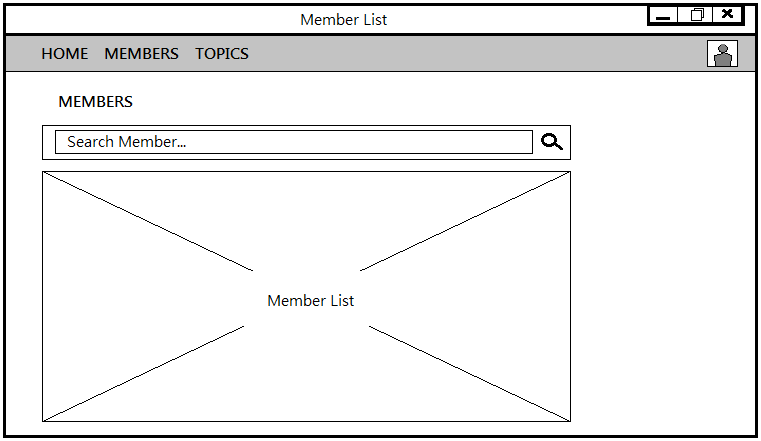
\includegraphics[width=.7\textwidth]{img/prototype/MemberList.png}
\caption{Prototype -- 使用者列表頁面(含搜尋功能)}
\label{pic:pro:memberList}
\end{figure}

\begin{figure}[H]
\centering
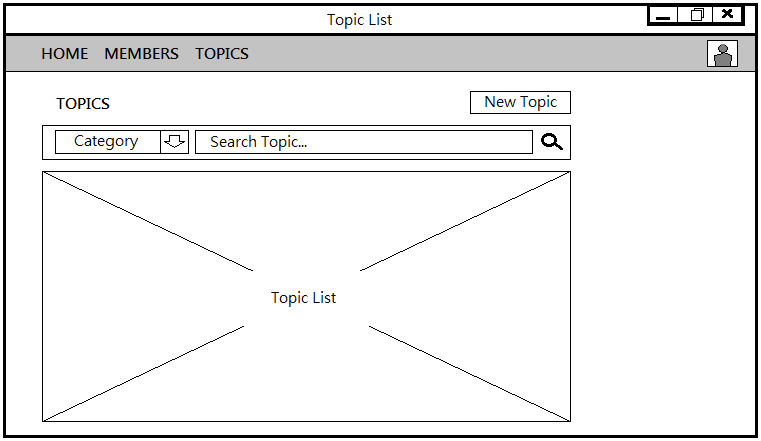
\includegraphics[width=.7\textwidth]{img/prototype/TopicList.png}
\caption{Prototype -- 文章列表頁面(含搜尋功能)}
\label{pic:pro:articleList}
\end{figure}

%% ####################### %%
\subsubsection{關係建立模組}

本系統中基於完成使用者之特定隱私權設計之理念,將在系統中提供建立好友關系的功能,也就是本模組的核心。本模組必須要能傳遞使用者的交友邀請、記錄使用者對於要求的回應與記錄使用者與其他用戶之關係。除了雙向之好友功能,本系統亦提供建立單項之關注其他使用者之功能。兩者的差異在於,好友是需要雙方合意,而可以使雙方看到對方之所有資訊;另一方面,關注關係不需要被關注者之同意,而系統僅於被關注者有發表新文章時會寄發通知信予關注者。本模組著重的重點在於資料抽象化之設計,更多細節請參考小節~\ref{sssec:following} 。

%% ####################### %%
\subsubsection{討論區模組}
討論區模組需包含以下三點功能:新增文章、瀏覽文章、標示文章類別。在新增文章時使用者將被要求選擇文章類別,以供其他使用者快速過濾想閱讀之訊息。由於系統沒有自動根據文章內容判斷其真實內容之能力,目前仍需仰賴使用者自動自發之行為來維持正確性,未來若能發展出足以將此行為自動化之方法則可降低系統在本問題之人力需求。此模組需同時提供標示文章類別與讓使用者方便瀏覽之功能,以達訊息交流之初衷。本模組將由前端網頁系統負責,只有將文章記錄至資料庫的行為需要後端資料系統輔助。

\begin{figure}[H]
\centering
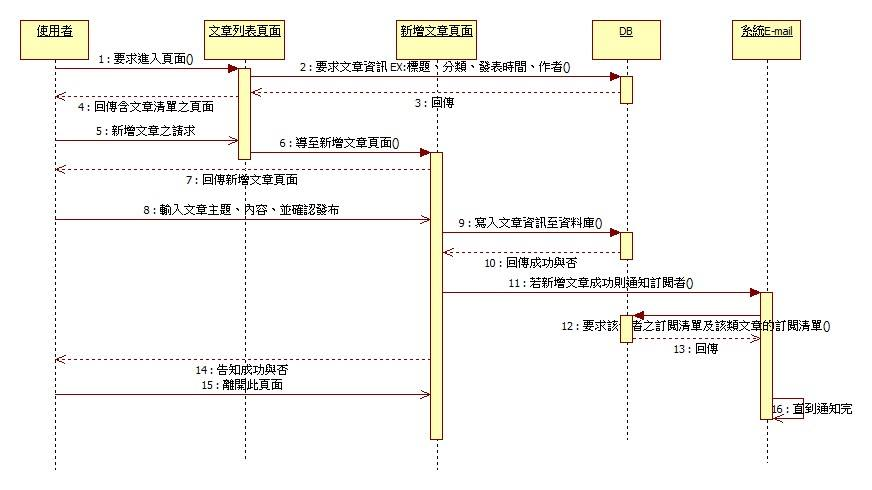
\includegraphics[width=1.05\textwidth]{img/useseq/stage2/seqNewArticle.jpg}
\caption{Sequence Diagram -- 新增文章}
\label{pic:seq:newArticle}
\end{figure}

\begin{figure}[H]
\centering
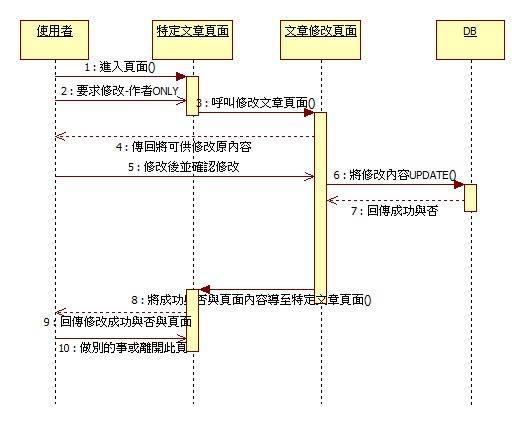
\includegraphics[width=.8\textwidth]{img/useseq/stage2/seqEditArticle.jpg}
\caption{Sequence Diagram -- 修改文章}
\label{pic:seq:editArticle}
\end{figure}

\begin{figure}[H]
\centering
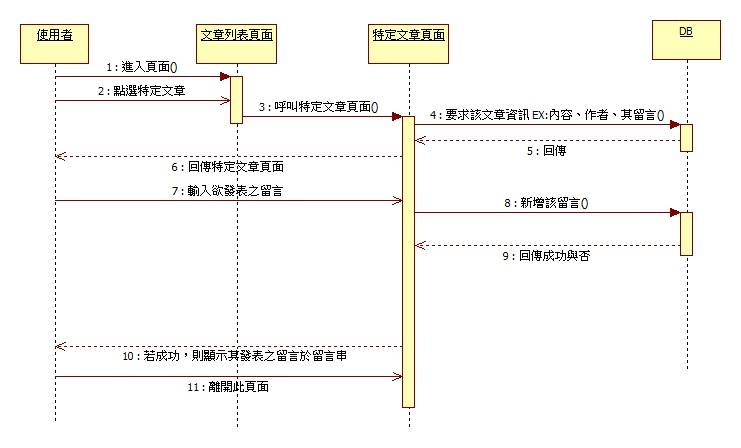
\includegraphics[width=1.05\textwidth]{img/useseq/stage2/seqNewComment.jpg}
\caption{Sequence Diagram -- 新增留言}
\label{pic:seq:newComment}
\end{figure}

%% ####################### %%
\subsubsection{訂閱模組}
\label{sssec:subscription}
訂閱模組中包含訂閱文章及訂閱文章類別等功能。訂閱之行為一致為當訂閱之目標有了內容之新增與改變時,將由後端信件系統發信至訂閱人所登記之信箱提醒使用者。訂閱文章的訂閱隊項為單篇文章,訂閱方法可包括在該文章留言或是點選訂閱按鈕,資料的改變為該文章被新增了評論時提醒。訂閱文章類別則將在任何一篇文章被標示為該類別時提醒使用者。本模組需由前端網頁系統展現、後端資料系統記錄與後端郵件系統共同合作完成。訂閱文章及文章分類請參考圖~\ref{pic:seq:search} 。

\begin{figure}[H]
\centering
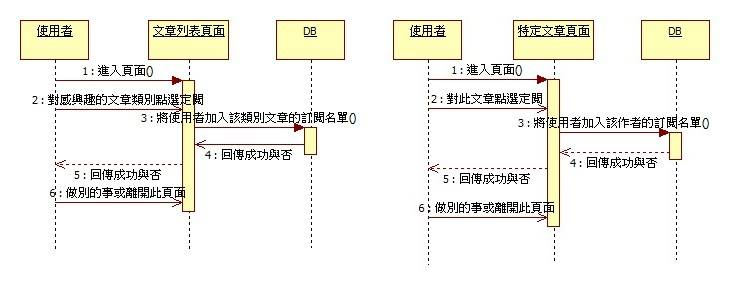
\includegraphics[width=\textwidth]{img/useseq/stage2/seqSearch.jpg}
\caption{Sequence Diagram -- 訂閱文章或文章分類}
\label{pic:seq:search}
\end{figure}



%% ####################### %%


%% ####################### %%
% first column
\begin{minipage}[t]{0.5\textwidth}
\subsubsection{API模組}

本系統基於 Grape,一個 REST-like API micro-framework,與 Ruby on Rails 整合,來提供系統 JSON API,並遵循 REST (Representational State Transfer) 的軟體架構風格實作,客戶端的應用通過 URI 來獲取資源的表徵,收取以 JSON 之資料格式來產生狀態的變化,對資源的操作包括獲取、創建、修改和刪除資源,這些操作對應於HTTP協議提供的 GET、POST、PUT 和 DELETE 方法。 以新增議題為例:當使用者需要新增議題時,透過客戶端程式來以 HTTP request Server,因為新增文章代表需創建新的資料,所以使用 POST 做為 HTTP request 的方法,並對其設定的URI(http://alumnibook.com/api/topics/)做 request,這樣 Server 就會判斷其 HTTP requset 參數來做相對應的回覆,若所夾帶參數通過檢驗即可建立新的議題,並回覆新增之議題的資料,若所夾帶參數未能通過檢驗,例如必須欄位未提供或是其資料格式錯誤,則會回傳錯誤訊息,API 所回傳的資料格式皆以 JSON 作為主要資料格式。API 最主要可以提供其他網站服務或是行動裝置端的程式使用,例如說圖~\ref{pic:seq:appi} 呈現了以手機程式為客戶端時,該服務與本系統之 API 之間可能的互動模式。
\end{minipage}
%second column
\begin{minipage}[t]{0.5\textwidth}
\begin{figure}[H]
\centering
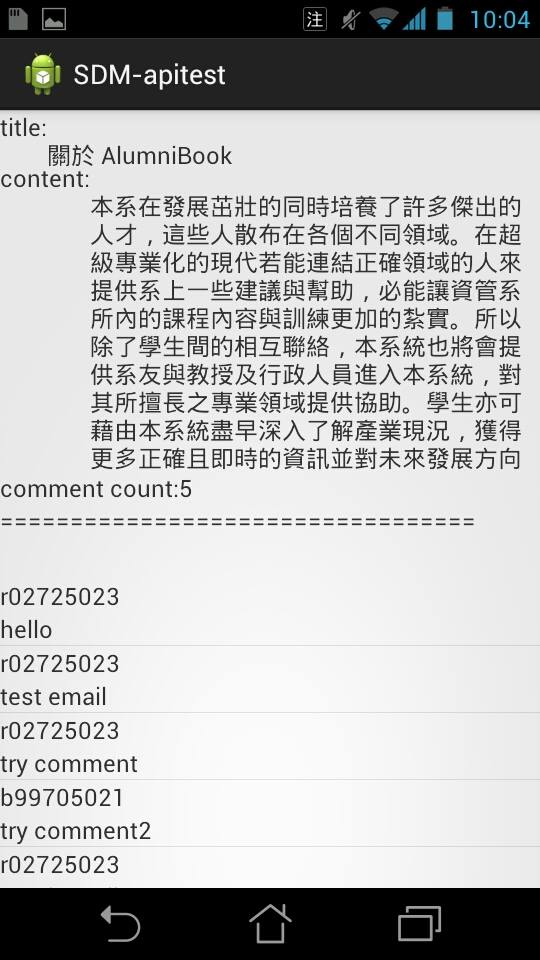
\includegraphics[width=0.65\textwidth]{img/prototype/android.jpg}
\caption{Android Screenshot -- 行動程式}
\label{pic:app}
\end{figure}
\end{minipage}

\subsubsection{行動程式}
行動裝置端的程式極其輕便,僅帶來快速的文章流覽功能。手機程式的執行畫面雛形如圖~\ref{pic:app} 所示。在手機端程式啟動後,程式會向API要求資料。在接收到伺服器端所提供的JSON陣列後,手機端會做一連串的處理動作。從該JSON陣列中一項一項抽取出來的資料在成功解構後會暫時以方便取用的格式放在本機端以供未來使用,並且先將使用者列表簡單的呈現給使用者。使用者選擇有興趣的文章時則可從本機端的資料中取得該篇文章的內文、作者以及評論。手機端程式與網站 API 之間的互動細節請參考圖~\ref{pic:seq:appi}。

\begin{figure}[H]
\centering
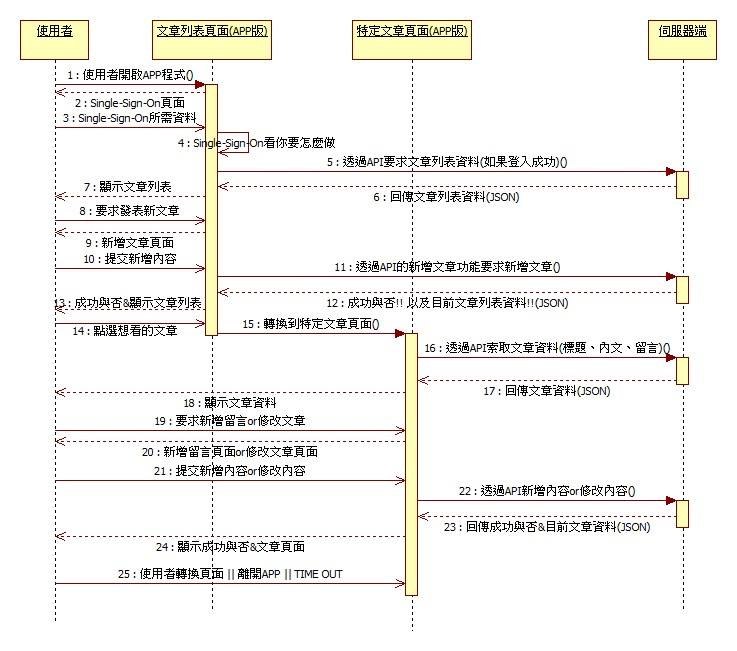
\includegraphics[width=\textwidth]{img/useseq/appi.jpg}
\caption{Sequence Diagram -- API and Android App}
\label{pic:seq:appi}
\end{figure}




\subsection{使用套裝軟體及開發工具、程式語言}
本系統採用 Ruby on Rails 作為主要伺服器端開發架構,使用 Ruby 2.0.0-p247 版本,Rails 4.0.0 版本,以 Grape 這個 Ruby REST-like API micro-framework 建立起主要 API server,提供網頁端與手機 JSON API,連結 MySQL(5.5.29) 資料庫儲存索取更新並維持資料正確與一致性,前端網頁頁面以 HTML5(HTML, CSS, JavaScript) 撰寫而成,採用Angular.js(1.2.0) 一個前端 JavaScript MVC 架構增加程式碼模組化與維護性,使用介面以 Bootstrap(3.0.0) 作為主要網頁前端外觀元件框架,加速雛形開發。
\subsection{系統環境需求}
目前Ruby on Rails Server架設在 Heroku 一個雲端應用平台,提供高度延展性,以亞馬遜 AWS EC2 為基礎建構而成的伺服器叢集,使用 git 上傳即可快速部屬,伺服器主要需要運行在 Ruby 2.0.0 與 Rails4.0.0 環境下。網頁前端頁面則放置在 Http server (如 Apache, Nginx) 下,並與 MySQL 資料庫放在資管系主機。前端網頁則相容於多數瀏覽器 (Chrome, Safari, Firefox…),提供使用者多樣的使用選擇。

\end{document}
